\documentclass[A4paper,11pt]{marine_2023_Paper}
\usepackage{graphicx}
\usepackage{amsmath}
\usepackage{amsfonts}
\usepackage{amssymb}
\usepackage{titlesec}
\titleformat{\section}[block]
{\normalfont\bfseries\filcenter}
{\thesection.}{.5em}{\bfseries}

\pagestyle{plain}



\title{Instructions to Prepare a Full Paper for the X International Conference on Computational Methods in Marine Engineering MARINE 2023}

\author{First A. Author$^{1*}$, Second B. Author$^{\dag}$ and Third C. Author$^{\dag}$}

\heading{First A. Author, Second B. Author and Third C. Author}

\address{$^{1}$ International Center for Numerical Methods in Engineering (CIMNE),
Universidad Polit\'{e}cnica de Catalu\~{n}a,
Campus Norte UPC, 08034 Barcelona, Spain,
e-mail: congress@cimne.upc.edu, web page: http://www.cimne.com/
\and
$^{\dag}$ Spanish Association for Numerical Methods in Engineering (SEMNI),
Edificio C1, Campus Norte UPC,
Gran Capit\'{a}n s/n, 08034 Barcelona, Spain,
e-mail: semni@cimne.upc.edu - Web page: http://www.semni.org\\[.5cm]
$^{*}$ Corresponding author: First Author, First.Author@cimne.upc.edu}

\newcommand{\V}[1]{\boldsymbol{#1}}
\newcommand{\nn}{\nonumber}
\newcommand{\D}[2]{\frac{\partial #1}{\partial #2}}

\begin{document}
\maketitle
\thispagestyle{empty}
\setlength{\parskip}{0.3cm}

\begin{center}{\bf ABSTRACT}\end{center}

Authors should use this document as a template. The Title is mixed case (initial capitals followed by lower case on all words except articles, conjunctions, and prepositions, which should appear entirely in lower case). The Abstract is a brief description of the entire paper, including the scope, the methodology and the key conclusions. It should be no longer than 250 words. The Abstract is followed by a list of up to six keywords, each separated by semi column. The Nomenclature follows after the list of keywords. Symbols should be in italic and listed in alphabetical order. First include Roman symbols, then Greek symbols, and finally the list of acronyms in Roman font. When the subscripts are made of more than one letter, use Roman font, otherwise use Italic (for example, I\_beam and I\_x). The units of all symbols should be included in squared brackets without using fractions and separated by a space (for example, m s-1), while acronyms should not have units and should not be used in equations.

\noindent {\bf Keywords}: keyword 1; keyword 2; keyword 3; keyword 4; keyword 5; keyword 6.

\section*{NOMENCLATURE}

\begin{tabular}{ll}
 $C_x$ & Aerodynamic force coefficient in the $x$-direction [-]\\
 $D_{ij}$ & Shear stress tensor [Pa]\\
 $\boldsymbol{F}$ & Aerodynamic force vector [N,N,N]\\
 $F_x$ & Aerodynamic force in the $x$-direction [N]\\
 $I_{\mathrm{beam}}$ & Area moment of inertia of the beam [m${}^{4}$]\\
 $p$ & Hydrostatic pressure [Pa]\\
 $U_{\infty }$ & Free stream velocity [m s${}^{-1}$]\\
${\tau }_x$ & Skin friction in the $x$-direction [Pa]\\
 $\rho $ & Fluid density [kg m${}^{-3}$]\\
 CFD &Computational Fluid Dynamics\\
 EFD &Experimental Fluid Dynamics
\end{tabular}

\section{INTRODUCTION}

This is the first section in the main body of the text after the Nomenclature. Please assure that a comprehensive critical review of the relevant literature is included. When necessary, use Column Break to avoid finishing a page with a heading.

\section{SUBMISSION REQUIREMENTS}

The manuscript should be prepared in Microsoft Word or Latex using this template or the Latex companion. A PDF version of the manuscript can be submitted.

Articles must be written either in American or British English. Articles that have been carefully proofread will be accepted for review, while articles that are clearly unacceptable will be returned to the Author(s) without being reviewed.

There is no limitation to the maximum number of pages.

Articles must be original, must not have been published previously or be pending publication anywhere else, and cannot be under review by any other forum.

Metadata underpinning the results, and additional material such as, for instance, videos and simulations, can be submitted in separate files and will be made available together with the electronic version of the paper on the conference website. Metadata and additional material will not be peer reviewed.


\section{DOUBLE BODY MODEL}
The hydrodynamic interaction force between a ship and other ships, the seabed, banks or fixed structures is strongly related to pressure changes due to increased or decreased flow velocity around the ship. The physical problem resembles that of a Venturi pipe. A mathematical model for calculation of a ships hydrodynamic interaction forces should capture the the Venturi pipe effect between the ships. Fortunately thats excately what the \emph{double body flow model} does. In the double body flow model is to assume that the free surface is flat and the body is mirrored the body and solution around
the still water level.
The double body flow model is based on potential flow theory, hence the water is assumed to be in-
compressible, inviscid and irrotational, and where the fluid velocity is the gradient of the velocity potential $\V{u} = \nabla \phi$. 
Mass conservation is satisfied through the Laplace equation for the velocity potential
\begin{equation}
	\nabla^2 \phi = 0, \quad z \in [-h,\eta],
\end{equation}
where $h$ is the sea depth and $z = 0$ is still water level. At the seabed the no-flux boundary condition applies
\begin{equation}
	\V{n} \cdot \nabla \phi = 0, \quad z = -h, 
\end{equation}
where $\V{n} = [n_x, n_y, n_z]^T$ is the normal vector to the seabed, pointing out of the fluid and into the seabed. Likewise are submerged bodies subject to the no-flux boundary condition
\begin{equation}
	\V{n} \cdot \nabla \phi = n \cdot \V{V} , \quad (x, y, z) \in S_B, 
\end{equation}
where $\V{n}$ is the normal vector pointing out of the fluid and into the body, $\V{V} =\V{u}_B + \V{\omega}_B \times \V{r}$ and $\V{u}_B$ and $\V{\omega}_B$ are the linear and rotational velocities of the body, $\V{r}$ is the direction vector from $CG$ and $S_B$ is the submerged surface of the body. A ship navigating in an open sea has the far-field boundary condition [9]
\begin{equation}
	\phi = \mathcal{O} (\sqrt{x^2 + y^2}) \quad \mathrm{for} \quad x^2 + y^2 \rightarrow \infty. 
	\label{eq_farfield}
\end{equation}
Conservation of momentum of a inviscid and irrotational fluid flow is described by the Bernoulli equation. In a ship fixed moving frame of reference, where the Bernoulli constant is zeros due to the far-field condition \eqref{eq_farfield}, it is
\begin{equation}
	p(x, y, z) = -\rho \left(\D{\phi}{t} -\V{V} \cdot \nabla \phi + \frac{1}{2} \nabla \phi \cdot \nabla \phi + gz \right).
	\label{eq_bernoulli}
\end{equation}
The hydrodynamic force on the submerged body is
\begin{equation}
	\V{F} = \int_{S_B} p(x, y, z) ~\V{n} dS.
	\label{eq_hydrodynamic_pressure_force} 
\end{equation}

\subsection{Linearization and pertubation expansion}
First we Taylor expand the velocity potential around the still water level, $z_{SWL}$,
\begin{equation}
	\phi(x,y,z) = \phi(x,y,z_{SWL}) + \eta \left.\D{\phi}{z}\right|_{x,y,z_{SWL}} + \mathcal{O}(\eta^2),
	\label{eq_phi_tay_exp}
\end{equation}
where the free surface elevation is $\eta = z-z_{SWL}$. Secondly, both the velocity potential and free surface elevation are perturbation expanded due to a small parameter $\varepsilon$
\begin{align}
	\phi = \phi_0 + \varepsilon \phi_1 + \mathcal{O}(\varepsilon^2), \label{eq_phi_per_exp} \\
	\eta = \eta_0 + \varepsilon \eta_1 + \mathcal{O}(\varepsilon^2).\label{eq_eta_per_exp}
\end{align}
Insertion of the expansions \eqref{eq_phi_tay_exp}, \eqref{eq_phi_per_exp} and \eqref{eq_eta_per_exp} in the Bernoulli equation \eqref{eq_bernoulli} and keeping only the zero'th order terms gives
\begin{equation}
	p(x, y, z) \approx -\rho \left(\D{\phi_0}{t} -\V{V} \cdot \nabla \phi_0 + \frac{1}{2} \nabla \phi_0 \cdot \nabla \phi_0 + gz \right),
	\label{eq_bernoulli_exp}
\end{equation}
and evaluation of this at the free surface, where the atmospheric pressure is assumed to be zero, and keeping only the zero'th order terms gives
\begin{equation}
	\eta_0 =  \frac{1}{g} \left(\D{\phi_0}{t} -\V{V} \cdot \nabla \phi_0 + \frac{1}{2} \nabla \phi_0 \cdot \nabla \phi_0\right).
\end{equation}
Now the surface integral for hydrodynamic force is split into the part under $SWL$ and the variation from $SWL$ due to $\eta$
\begin{align}
	\V{F} &= \int\limits_{S_{B,SWL}} p(x, y, z) ~\V{n} dS + \int\limits_{ S_B\backslash S_{B,SWL}} p(x, y, z) ~\V{n} dS.
\end{align}
The latter integral is simplified by insertion of the expanded pressure \eqref{eq_bernoulli_exp} and the vertical integration limits from $z_{SWL}$ to $z_{SWL}+\eta_0$
\begin{align}
	\V{F} &= \int\limits_{S_{B,SWL}} p(x, y, z) ~\V{n} dS + \frac{1}{2}\rho g\int  \eta_{0,y<0}^2 ~dx- \frac{1}{2}\rho g\int\eta_{0,y>0}^2 ~ dx.
\end{align}



\subsection{Sub-Headings}

Sub-headings are numbered, mixed case (initial capitals followed by lower case on all words except articles, conjunctions, and prepositions, which should appear entirely in lower case), and bold.

\subsubsection {Additional Sub-Headings}

Additional sub-headings should be numbered, mixed case and bold.

\section{ARTICLE FORMAT}
\subsection{Page Setup and Page Numbers}

The margins of this template are as in Table 1. The page numbers format is as in Table 2.

\subsection{Equations}

Equations must be included using the command Equation in the tab Insert. Please use punctuations as appropriate together with the equations (see examples below). Equations should be numbered consecutively using numbers enclosed in parentheses. The equation number can be added including \# followed by the equation number between parentheses at the end of the equation. For example, within the Equation environment, typing a=b,\#(1) and hitting return results in:
\begin{equation}
Ax = b
\label{eq1}
\end{equation}
where the meaning of each symbols such as $a$ and $b$ should be defined in the text before or immediately after, such as here, when they are used for the first time. Another example is as follow. The drag coefficient, which is defined as
\begin{equation}
C_D=\frac{1.328}{\sqrt{Re_L}},
\label{eq2}
\end{equation}
depends on the Reynolds number, $Re_L$, based on the ship length $L$.

 Use the Equation environment also in the main text to avoid that the symbols appear with different fronts in the equation and in the text (for example, $a$ vs a, and $L$ vs L). Every symbol must also be included in the Nomenclature at the beginning of the article.

\subsection{Tables}

 Tables are numbered consecutively and captioned. The caption title is bold followed by full stop (e.g. \textbf{Table~1}), all caption is 11 points and centered above the table.

 The body of the table is 11 points. Tables are positioned within the body of the article, centered, and as close as possible to the place where they are first discussed. Bold and colored shading can be applied.

 \begin{table}[h!]
\caption{This is an example of a table showing the template margins.}
\begin{center}
\begin{tabular}{{l}p{0.2in}{l}}
Top & &2.5 cm \\
Bottom && 2.5 cm \\
Left && 2.0 cm \\
Right && 2.0 cm \\
Gutter && 0.0 cm \\
Header && 1.0 cm \\
Footer && 1.0 cm \\
\end{tabular}
\end{center}
\end{table}

\begin{table}[h!]
\caption{Page numbers format.}
\begin{center}
\begin{tabular}{lp{0.2in}l}
Position & &Bottom of the Page \\
Alignment & &Center \\
Number on first page && Yes \\
First page number && 1 \\
\end{tabular}
\end{center}
\end{table}

\subsection{Figures}

 The Author should make every effort to include figures of memory size small enough so that the document size is manageable for downloading and opening over the internet and, at the same time the resolution of the figures is adequate for printing.

 All figures should be numbered consecutively and captioned. The caption should be 11 point bold, placed below the figure (as opposite to table captions that are placed above the table).

 Figures should be positioned within the body of the article, centered, and as close as possible to the place where they are first discussed. Wrapping style should be ``in line with text''. Color graphs, photos and animations are encouraged.

 IMPORTANT: text within the figure should be no smaller than 9 points, and the symbols should appear with the same font type as in the Nomenclature.

 Equations, figures and tables can be referenced in the text such as, for instance, equation 1, Eq. 1, Eqs. 1 and 2, Eqs. 1-3, Fig. 1, Figs. 1a and 1b (for multiple sub-figures), Tab. 2, \textit{etc. }

 When necessary, use Column Break to keep the caption with its table or figure on the same page.

\begin{figure}[t]
\centering
%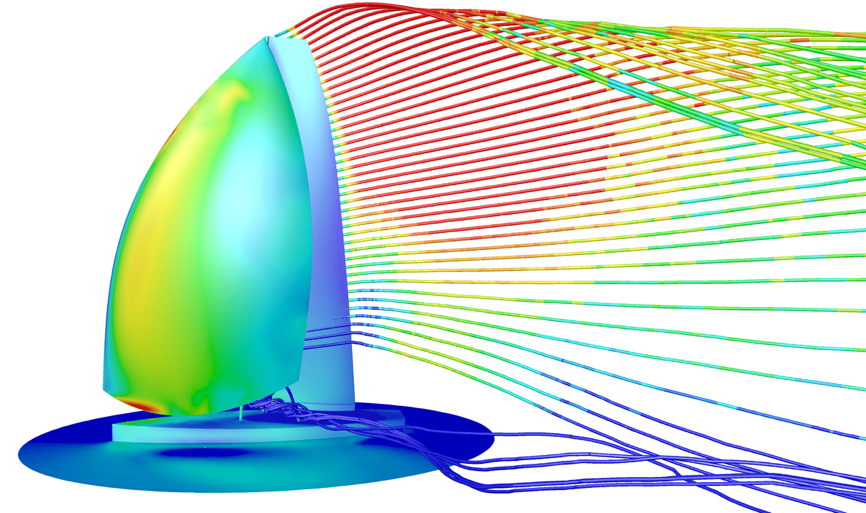
\includegraphics[width=11cm]{fig-example.eps}
\caption{Example of a figure.}
\label{fig1}
\end{figure}

\subsection{Citations}

 When the citation is part of the sentence, the citation includes the Author's last name and, between parentheses. For example, Bowman (1988) showed that this is a good citing style. Conversely, when the citation is not part of the sentence, then also the Author's name is within parentheses  (Bowman, 1988). Append lower-case letters to the year in cases of ambiguity (Bowman, 1989a). Multiple Authors are treated as Bowman and Skipper (1988) when there are two Authors and, in the case of three or more Authors, we list only the first Author followed by \textit{et al. }in italic. For example, see Bowman \textit{et al.} (1988). Multiple citations that are not part of the sentence should be separated by semicolons  (Bowman 1989; Skipper 1990).

\subsection{Inquiries}

 If you have any questions about the preparation or submission of your article as instructed here, please send an email to marine@cimne.upc.edu.


\section{CONCLUSIONS}

 It is recommended that the main body of the text ends with a summary of the key conclusions. This section may include a summary of the scope and of the methodology of the article, and a detailed list of conclusions in order of importance.

\section*{ACKNOWLEDGEMENTS}

 Every fund that supported the research must be acknowledged. Brief personal acknowledgements may also be added. For example, ``this work received funds from the European Research Council (grant no. XXXXXX). The authors are especially grateful to the Reviewers for their help in improving the article. This section can be skipped if the research has not received any financial contribution.

 \section*{AUTHOR'S CONTRIBUTION}

 This section is not compulsory. Authors can consider to identify their contribution to the reaserach project and the preparation of the manuscript. Example text is as follow. ``FAA designed the experiments, processed the data, and wrote the first draft of the manuscript. FAA and SBA undertook the experiments and processed the data. TCA supervised and coordinated the project. All authors edited and approved the manuscript.''


\section*{REFERENCES}
All references cited in the text should be listed at the end of the article in alphabetical order.

Bowman, A. B. (Year). Book Title (italic, initial capitals followed by lower case on all words except articles, conjunctions, and prepositions, which should appear entirely in lower case). Publisher, city, country.

Bowman, A. D. and Skipper, E. F. (Year). Title of Journal Article (roman font, initial capitals followed by lower case on all words except articles, conjunctions, and prepositions, which should appear entirely in lower case). Journal Name (in italic), volume (number), pages.

Bowman, A. D. and Skipper, E. F. (1988). Title of Journal Article. Journal of Sailing Technology, 2, 1-31.

Bowman, A. D., Skipper, E. F. and Pitman, J. K. (Year). Title of Conference Article. Proceedings of Conference Name (in italic), dates, city, country.

Bowman, A. D., Skipper, E. F. and Pitman, J. K. (1988). Title of Conference Article. Proceedings of Conference Name, March 15-16, Annapolis, MD, USA.

Larsson, L., Eliasson, R. and Orych, M. (2014). Principles of Yacht Design. Adlard Coles Nautical, London, UK.

\end{document}


